\section{Metodologia SFC: Uma breve introdução}
\label{IntroSFC}
%TODO: Não recomeçar nota de rodapé


A presente seção tem por objetivo apresentar as etapas e procedimentos da metodologia  SFC\footnote{Para uma análise mais pormenorizada das linhagens da abordagem SFC, ver \textcite{caverzasi_stock-flow_2013}.}. De forma bastante sucinta, tal metodologia é composta de três procedimentos: (i) determinação da estrutura contábil; (ii) exposição das equações comportamentais e; (iii) solução. Dito isso, a figura \ref{Resuminho} pretende resumir as etapas mencionadas e explicitar a diferença entre a \textit{metodologia} SFC um \textit{modelo} SFC seguindo alguma linhagem teórica. 


\begin{figure}[htb]
	\caption{Resumo esquemático da Metodologia SFC}
	\label{Resuminho}
	\centering
	\begin{tikzpicture}
	[node distance = 1cm, auto,font=\footnotesize,
	% STYLES
	every node/.style={node distance=3cm},
	% The comment style is used to describe the characteristics of each force
	comment/.style={rectangle, inner sep= 5pt, text width=4cm, node distance=0.25cm, font=\scriptsize\sffamily},
	% The force style is used to draw the forces' name
	force/.style={rectangle, draw, fill=black!10, inner sep=5pt, text width=4cm, text badly centered, minimum height=1.2cm, font=\bfseries\footnotesize\sffamily}] 
	
	% Draw forces
	\node [force] (rivalry) {Hipóteses};
	\node [force, above of=rivalry, fill=red!70] (substitutes) {Equações comportamentais};
	\node [force, text width=3cm, dashed, left=1.5cm of substitutes,fill=blue!50] (state) {Metodologia SFC};
	\node [force, left=1cm of rivalry] (suppliers) {Estrutura contábil};
	\node [comment, below=0.25 of suppliers] (comment-suppliers) {Relação entre lado real \\e financeiro};
	\node [force, right=1cm of rivalry] (users) {Solução};
	\node [force, right=1cm of substitutes, dashed, fill=purple!50 ] (PK) {Modelo \\ $\bullet$ --SFC};
	%	\node [force, below of=rivalry] (entrants) {Threat of new entrants};
	
	%%%%%%%%%%%%%%%
	% Change data from here
	
	% RIVALRY
	\node [comment, below=0.25 of rivalry] (comment-rivalry) {Cambridge/New Cambridge\\
		Kaleckiano\\
		\textbf{Supermultiplicador Sraffiano}};
	
	
	\node [comment, below=0.25 of users] {Analítico\\
		\textbf{Simulação}};
	
	
	% Draw the links between forces
	\path[->,thick] 
	(rivalry) edge (substitutes)
	(suppliers) edge (rivalry)
%	(rivalry) edge (users)
	(state) edge (substitutes)
	(state) edge (suppliers)
	(substitutes) edge (PK)
	(PK) edge (users);
	
	\end{tikzpicture}
	 
	\caption*{Fonte: Elaboração própria}
\end{figure}


As etapas contábeis da abordagem SFC são constituídas por\footnote{Esta seção não pretende expor a metodologia pormenorizadamente, mas sim expor seus procedimentos de modo a esclarecer as etapas que foram adotadas. Dito isso, a construção das matrizes a serem usadas fica a cargo da seção \ref{SecModelo}.}: (i) seleção dos setores institucionais e dos ativos a serem incorporados; (ii) mapeamento das relações dos fluxos entre os mencionados setores por meio da construção da matriz de fluxos; (iii) construção da matriz dos estoques de riqueza (real e financeira) em que são contabilizadas os ativos e passivos  bem como a posição líquida de cada setor; (iv) identificação das formas que os fluxos são financiados e sua respectiva acumulação nos estoques. Desse modo, o rigor contábil adotado faz com que o grau de liberdade, ou seja, com que a arbitrariedade do modelo diminua. 
Ao partir de um aparato analítico baseado em identidades contábeis, surgem restrições que precisam ser seguidas  --- como em todo modelo macroeconômico --- mas o que distingue a metodologia SFC das demais é a conexão do lado real com o financeiro de forma integrada\footnote{Vale destacar que as identidades contábeis são o ponto de partida, mas não são suficientes para garantir a consistência do modelo. Exemplo disso pode ser visto na exposição de  \textcite[p.~27--8]{godley_monetary_2007}  a respeito da contabilização das ações que não são, legalmente, um passivo das firmas e, portanto, o pagamento de dividendos não é uma obrigação contratual. Apesar disso, considera-se que as ações emitidas pelas firmas são similares aos \textit{corporate bonds}, garantindo a consistência do modelo. O que pretende ser destacado é que por mais que tal simplificação seja razoável, não deixa de ser uma hipótese.}. 
%TODO Rever substituição de "liquidar" por "se endividar"
Dito isso e uma vez respeitadas as identidades contábeis, a soma da posição financeira líquida dos setores institucionais é zero. Tal procedimento garante que para que um setor acumule riqueza financeira, outro necessariamente se endivida e, assim, não existem ``buracos negros'' \cite{godley_money_1996}. 


Por mais que esta etapa seja centrada na contabilidade social, isso não implica que não possua um componente teórico associado\footnote{A título de exemplo, \textcite[p.~15--16]{macedo_e_silva_peering_2011}  pontuam que %estão presentes elementos pós-keynesianos\footnote{É importante ressaltar que se seguir a definição de \textcite{lavoie_post-keynesian_2015} em que estão incluídos autores sraffianos, os pontos elencados anteriormente deixam de ser consensuais.}:
	os agentes econômicos são categorizados de acordo com o tipo de estoque de riqueza que possuem.
}. 
% (i) os agentes econômicos são categorizados de acordo com o tipo de estoque de riqueza que possuem; (ii) os agentes celebram contratos que impactam sua riqueza e geram fluxos monetários que implicam novas mudanças na composição patrimonial desses agentes; (iii) ganhos e perdas de capital afetam o valor dos estoques que impactam na dinâmica do sistema; (iv) a composição patrimonial dos agentes e setores evolui de forma assimétrica de acordo com o grau de alavancagem, preferência pela liquidez/risco e (v) o acúmulo de ativos e passivos pelos agentes interfere na correlação de forças da economia. 
%Desse modo, por mais que a estrutura contábil parta das identidades, isso não a isenta de teoria. 
No entanto, por se tratar de identidades, nada de causal pode ser extraído delas. As relações de causalidade do modelo (agora modelo e não metodologia) decorrem das equações comportamentais que, respeitando a consistência, podem ser de qualquer linhagem teórica (\textit{e.g.} kaleckiana, sraffiana, etc.). A ênfase em tratar a abordagem SFC enquanto uma metodologia decorre da flexibilidade de incluir inúmeras teorias e propostas apesar da rigidez de seus procedimentos. Apenas para elencar (e não esgotar) alguns temas caros a heterodoxia, tal abordagem permite tratar as formas de financiamento das firmas; endogeneidade da moeda e importância do sistema bancário \cites{godley_money_1999}{lavoie_note_1999}; endividamento, distribuição de renda e financeirização \cites{dos_santos_revisiting_2009}{palley_inside_2010}{hein_finance-dominated_2012} e, apenas para restringir os temas; análises empíricas e proposições de política econômica \cites{godley_seven_1999}{godley_fiscal_2007}{godley_simple_2007}{arestis_income_2011}. 

A mesma variabilidade de temas passíveis de serem abordados pela metodologia SFC se estende para a pluralidade dos ativos e do grau de complexidade financeira de cada modelo. Uma forma de visualizar tal flexibilidade é por meio da figura \ref{Heatmap} em que são mapeados os ativos mais frequentes. No entanto, este gráfico também revela que a literatura não dá a devida atenção às residências\footnote{Deve ser pontuada a notória exceção de \textcite{zezza_u.s._2008} já discutida no capítulo \ref{CapTeorico}.}, sendo o ativo menos estudado. 


\begin{figure}[H]
	\centering
	\caption{Mapa de calor dos ativos modelados com SFC}
	\label{Heatmap}
	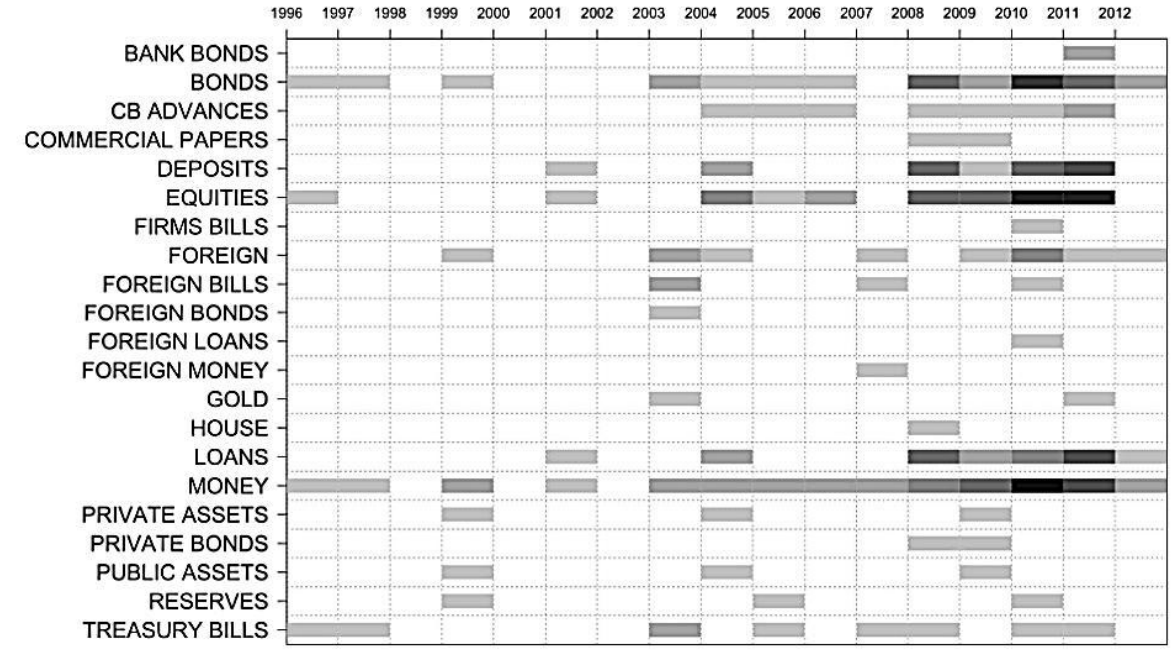
\includegraphics[width = 0.9\textwidth]{Modelo/Caverzassi_Heatmap.png}
	\caption*{\textbf{Fonte:} \textcite[p.~4]{caverzasi_stock-flow_2013}}
\end{figure}



%BREVE REVISÃO MODELOS SHIPMAN + GRÁFICO CAVERZASSI



Feitas essas ressalvas, dada a estrutura contábil, as hipóteses e as equações comportamentais, resta seguir para a solução do modelo. Como pontuam \textcite{caverzasi_stock-flow_2013}, existem duas vias: (i) simulação e (ii) analítica. A primeira delas permite expor de forma mais clara as relações entre as variáveis de modelos mais complexos em que a solução analítica não é facilmente encontrada (\textit{i.e.} sistemas intratáveis). No entanto, tal caminho fez com que o grau de complexidade dos modelos simulados fosse exponencializada de modo que as relações de causalidade tornam-se facilmente turvas. Diante destas complicações, o presente capítulo prioriza a parcimônia de modo que serão incluídos apenas os elementos necessários. A justificativa deste procedimento decorre da maior clareza da modelagem frente a um menor ``realismo''.
Além disso, tal postura permite encontrar soluções analíticas com maior facilidade de modo que são explicitados os parâmetros mais relevantes para as trajetórias de longo prazo. Apesar da parcimônia do modelo, a simulação tem a vantagem
de fornecer informações que não se restringem às soluções de equilíbrio e esta forma
também será selecionada para resolver o modelo uma vez que permite também analisar o \textit{traverse}.
Dito isso, a seção seguinte expõe o modelo que será simulado adiante.
%TODO Rever substituto de Médio prazo
